\section{Evaluation}
\label{sec:evaluation}
% comment by Daniel: This section could be used to provide information on the methodology, general issues, selection process of the upcoming issues (subsections) or similar...

In this section, we will first provide an evaluation of the AR gameplay components.
Secondly, we will talk about the movements of the demons in the game before evaluating the data analytics pipeline and the used OCR framework.
Finally, we will provide a short case study to evaluate the implemented game in a real-world environment.

% AR-Komponente (Bewegung des Dämons, Werden die PoI’s wiedergefunden, etc.)
% - biggest challenge: ensuring that tracking points at PoI remain consistent as user approaches; old visual context is lost as they focus e.g. on a single part of the desktop --> might cause ARCore to recalc coordinate system (could have been nice to pause allocation of tracking points and rely on accelerometer, but ARCore does not support this)
\subsection{Tracking Point Accuracy}
The most important limitation for the augmented reality subsystem we encountered was the stability of tracking points in the virtual space.
As described before, quick movement caused ARCore to lose track of many of the points and creating new ones, thus invalidating potentially crucial information about the room.
Since the setting of the game encourages the feeling of hunting after the demon, quick movements are unfortunately an expected and potentially necessary part of the game.
Further problems arose when the user moved closer towards a point of interest at which the demon was sitting.
As they approach the point, a lot of points all around the room will "disappear" as the frame of the camera narrows in on the area of interest.
This would not necessarily be a problem, however, ARCore will constantly recompute the coordinate system and make considerable corrections to the origin when it loses important tracking information or gets a lot of new points in an area.
Often, this had the effect of the demon getting farther and farther away from the player as they approach it, even though it appeared to be sitting at a constant position.

At the time of writing, ARCore does not expose an option to \enquote{freeze} the coordinate system.
This functionality would have likely remedied our issues if we froze the coordinate system when switching to the capturing phase, where stable positions are essential and relied on the phone's accelerometer and picture data to move the camera in the existing virtual space.
ARCore did not expose sufficient access to the lower level system for us to try this approach by ourselves, so we will either have to wait for its developers to add this functionality or use and modify an open source augmented reality framework to solve this specific use case.

% - by defining anchors on the relevant tracking points, ARCore will ensure most of the time that objects remain within reach -- timeout and fallback to showing spell even though user is not close enough otherwise
As a workaround to this issue, we make use of the ARCore anchors, which will update and move around the coordinate system to try and make up for changes to the coordinate system's origin or scale.
This helped most of the time to ensure that the demon will at least be within the activation distance for the capturing phase, but it still appeared to coast around the spot.
To not block the game altogether when the demon attaches to a point with incorrect depth, making it impossible for to the user to come close enough, we added a timeout that will move the game onwards in the hope that the next point may be better.

\subsection{Demon Movement}

% Comment from daniel: I would like to see lots of images here, e.g., show a stupid positioning due to errors, or how does good tracking accuracy compare to a bad one by example
\begin{figure}[ht]
    \centering
    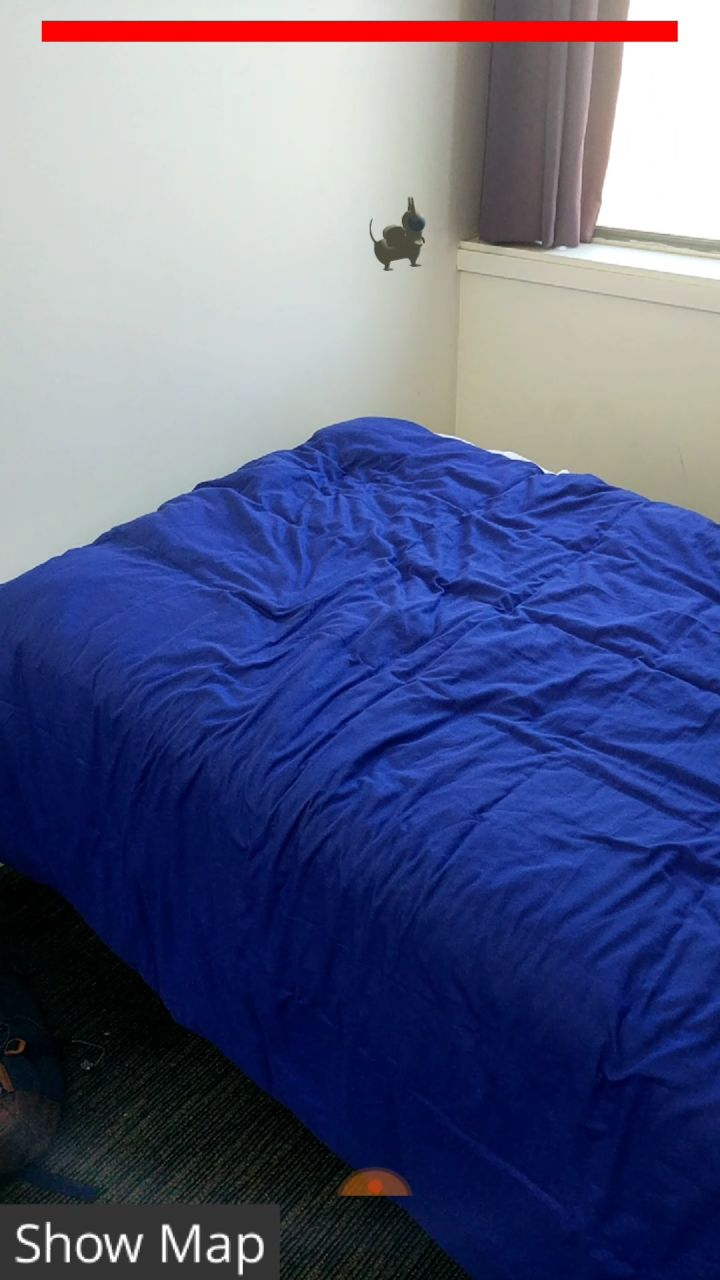
\includegraphics[height=8cm]{graphics/demon-wrong-depth.jpg}
    \caption{The demon appears to be floating inside the wall. The debug output in the console reported a distance from the camera of about 7 meters while this frame was captured. The distance from the camera to the wall is about 2 meters.}
    \label{fig:demon_wrong_depth}
\end{figure}

% - movement of demon feels weird at start, as dimensions of room are unknown
The movement of the demon in our current implementation is simplistic and makes next to no use of advanced possibilities, like collision detection.
This is mainly because the quality of the tracking points even for our room size estimation may vary greatly so that we chose to use the simplest possible primitive volume in 3D space to reduce the chance of the demon getting locked within non-existing obstacles that have been formed by errors in the tracking point estimation.

% - placement of waypoints close to user confuse, but as they traverse the room and turn frequently it's hard to predict where they will be
Our concept of exploring the room size by encouraging the user to turn frequently at the start of the session, by making the room very small, may lead to some confusion as the demon appears to travel through impossible ways, for example through the user.
As the room quickly grows bigger, this may not be as much of an issue, however, it may make sense to add a better waypoint system than simply selecting random points in the known space.
This may also help to make the demon feel like a more believable creature.

\subsection{Mobile Client Analysis}
The current concept and implementation of the data analysis pipeline does not recognize potential information in every scenario.
Firstly, the blurriness estimation is not very precise in some cases. For example, when using a shallow focus, some regions are completely focused, while others are very blurry. This will result in a low blurriness estimation, even though not many regions of the frame are usable.
Also, the detection of regions with potential information relies heavily on the contour detection.
This is not an ideal approach, as regions are disregarded if multiple contours overlap or if they are not clearly discernible from the scene background.
An example is the flyer in the foreground of \autoref{fig:cont_dect}. As we can see in \autoref{fig:cont_dect2}, the result of the canny filter allows no clear separation of the content due to the low contrast with the background.
Also, the current heuristic for determining the likelihood of textual information, the combination of noise and colorfulness estimation, is not able to differentiate between low-color, high-noise regions in general and actual text in particular. In \autoref{fig:estimators}, we can see that all three found contours have rather similar estimations. Even if the letter is still a bit more noisy than the other frames, all three contours would be good candidates.
Since we therefore employed an additional text detection step with support from the server, very small text could potentially be missed.
It might be advisable to move away from the contour-based approach and instead aggregate scores for small quadrants of the real-world coordinate system.
This would eliminate the additional round trip to the server, while presumably enabling the detection of regions that the EAST detection misses.

\subsection{OCR}
\emph{Tesseract}, the used OCR framework, is able to produce great results when used in scenarios where the graphical representation of the text has a high resolution, is not distorted and offers high contrast.
An ideal example would e.g. be a scan of a non-handwritten page of a book. \\
This immediately shows that \emph{Tesseract} is probably not the best framework to use in a real-world scenario where we have a lot of sparse text which is likely distorted because of wrong focus and fast camera movements. 
Of course, by preprocessing we can filter out frames which are too blurry, deskew and rotate distorted text as well as convert image to black and white in order to generate higher contrast. 
However, all those operations are not producing optimal solutions and can only improve the results slightly. 
Additionally, the issues of low resolution and unusual fonts let alone handwriting are impossible to be fully mitigated. 

\subsection{Case Studies}

\begin{figure}[htpb]
  \centering
  \subcaptionbox{Full view}{%
    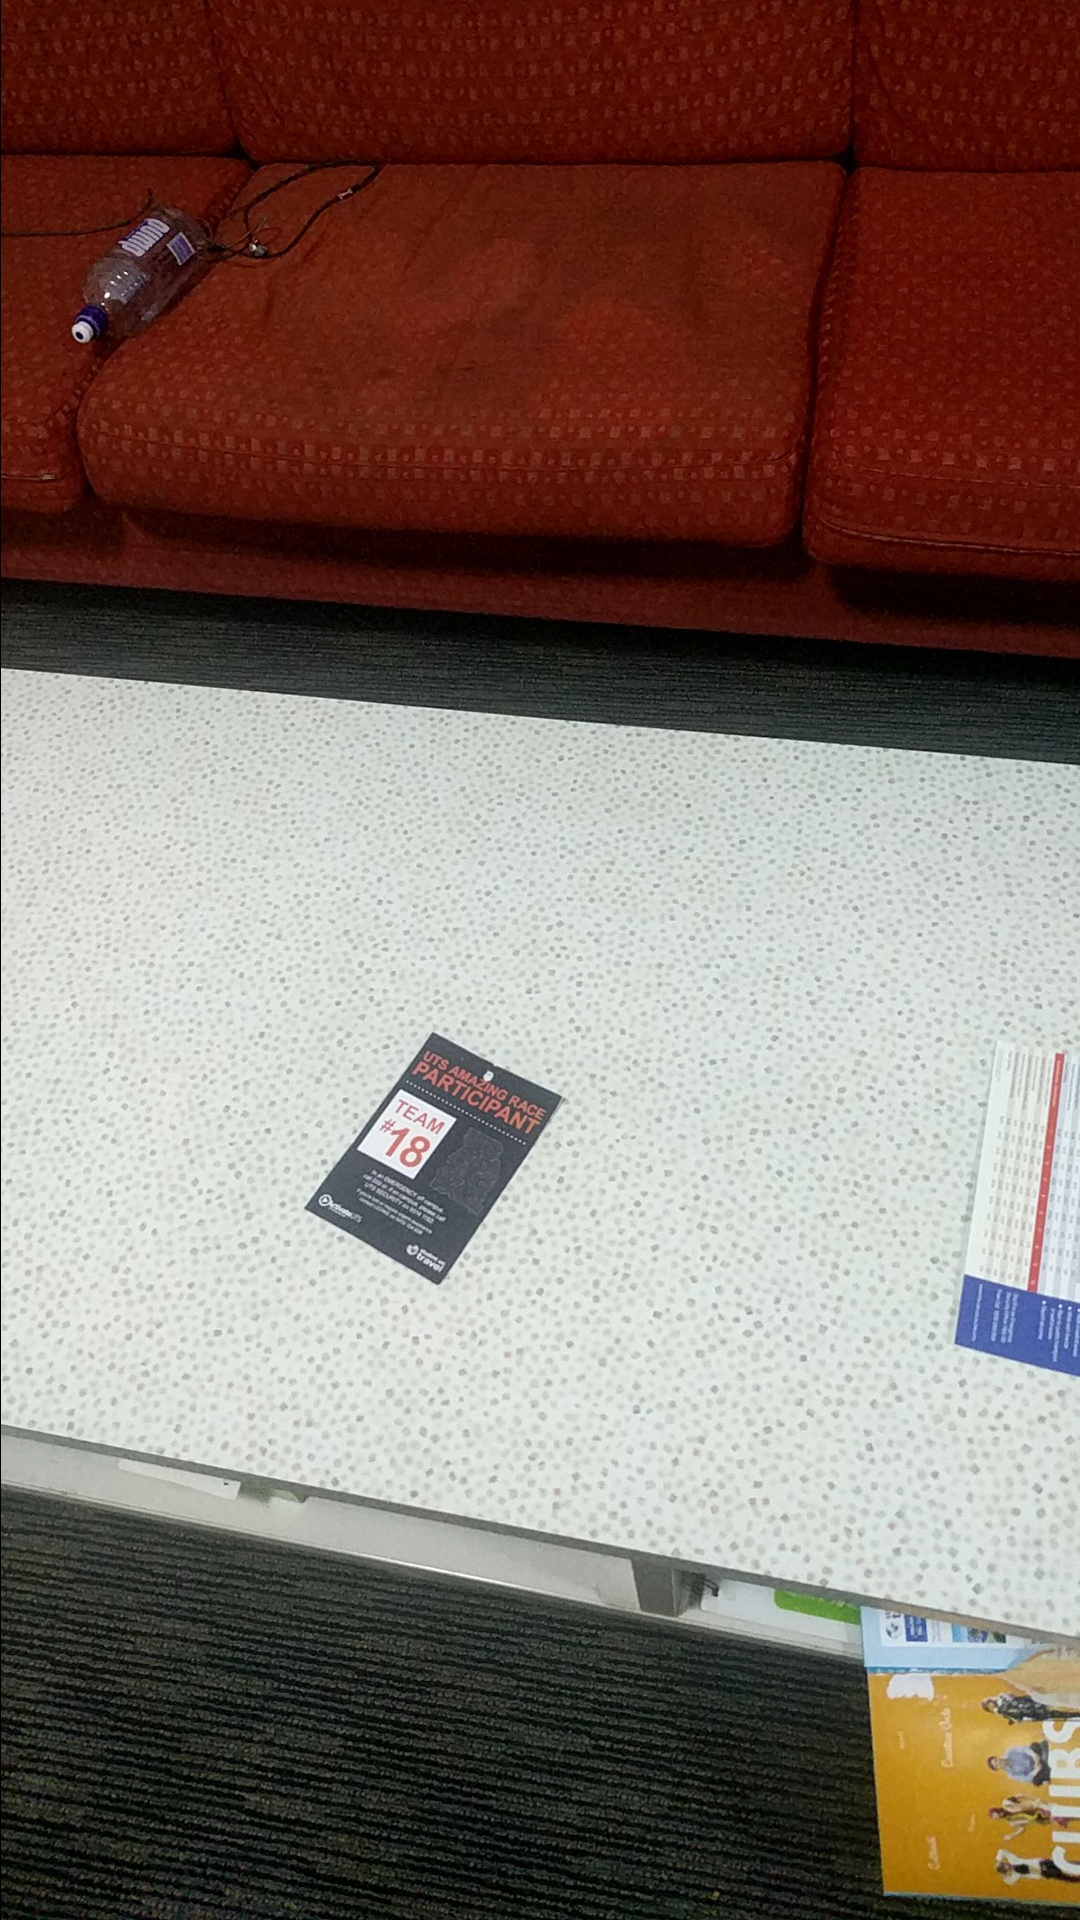
\includegraphics[width=4cm]{graphics/sticker-full.jpg}}\quad
  \subcaptionbox{Extracted part}{%
    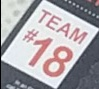
\includegraphics[width=3cm]{graphics/sticker-closeup.jpg}}
  \caption{The full view of the analyzed frame and the extracted part that was used for further analysis.}\label{fig:example-frame}
\end{figure}

We tried the capturing aspect with four different people, who had not seen the game before. They received three sentences of basic instructions (red ball, needs to be shot three times; will transform into a demon, to which you walk close by; then draw the pattern that appears to win the game). All four managed to complete a game without further instructions and played a total of eleven runs, two of which had to be aborted because the demon left the clipping volume. The gameplay took place in a large living room of around 6x8 meters squared.

The most notable problem in terms of gameplay was the loss of tracking information when the testers scanned the room rapidly and moved the camera to the plain white ceiling or quickly moved towards a part of the plain white wall. Best results were obtained when the testers held the camera tilted towards the floor for a longer while. This gave ARCore the opportunity to get a set of solid base points that it could find again when the camera moved nearby. Otherwise, when holding the camera at eye level or towards the ceiling, a larger area had to be analyzed and often led to points erroneously being detected as too far away.

\begin{figure}
    \centering
    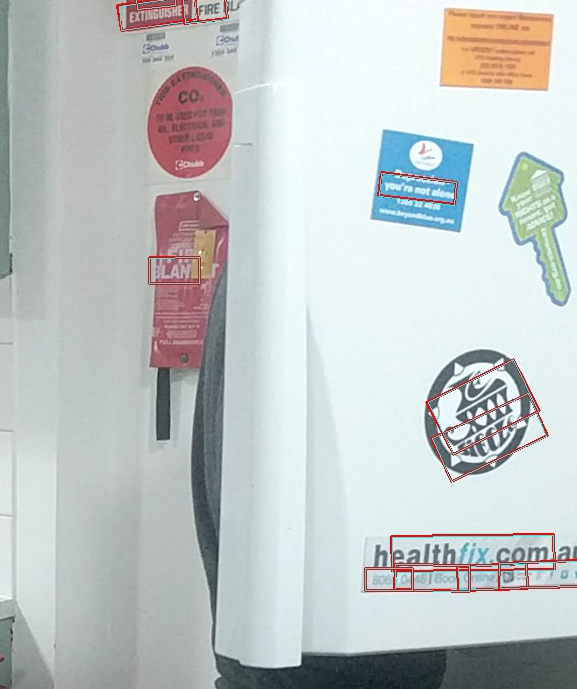
\includegraphics[height=8cm]{graphics/fridge.png}
    \caption{Part of the fridge door containing the text snippets that were found during one of the case study gameplay sessions. Marked with red rectangles are the areas that were recognized to contain text and analyzed by the OCR.}
    \label{fig:fridge}
\end{figure}

Four potential points of interest were placed in the room. See \autoref{fig:example-frame} for an example. During the eleven runs, the demon specifically targeted points of interest three times (the fridge in \autoref{fig:fridge}, the sticker in \autoref{fig:example-frame} and a pinboard on the wall). 
Twelve snippets of text could be recovered from pictures taken during the sessions, with some information successfully converted by the OCR, for example, the URL \enquote{healthfix.com.au} turned into the string \enquote{ealth/ix.com}, see \autoref{fig:fridge}.

These results reflect real usage by players that do not aim to help the data exploitation system.
They had no knowledge of this component and did not take particular notice of the planted points of interest.
In another test in a smaller room and a player that knew about the data exploitation aspect and that moving the camera along areas of low contrast should be avoided, results turned out a lot more positive, with the demon choosing points of interest at least once in three points, with the other two still being chosen randomly or at a place that did not contain textual information.
This also allowed recovering larger pieces of text, even though the quality of the translated strings is comparable, with letters being replaced by symbols and letters missing at the start or end of the string.
Results, as observed in this exploit-oriented usage, are comparable to those demonstrated in \autoref{sec:implementation-data-analysis}.


% Brand-Detection

% Scalability
